\chapter{Finanzas y primer teorema de asignación de precios}

Nos introducimos ahora en el mundo de las denominadas \textit{matemáticas financieras}. En las secciones anteriores hemos expuesto todas las herramientas matemáticas necesarias para el trabajo y en esta vamos a explicar los conceptos económicos o financieros. Una vez se haya completado este apartado estaremos dispuestos a enunciar y probar el enunciado culmen de este trabajo que nos servirá para la valoración de activos financieros en mercados finitos. \\

Nos preguntamos entonces: ``¿qué es un \textit{activo}?''. Un activo o título de valor se define como un recurso con valor que alguien posee con el fin de obtener un beneficio en el futuro. Podemos diferenciar entre activos seguros, como depósitos en el banco o bonos del estado, y activos con riesgo, como las acciones. Uno de los conceptos más importantes que tenemos es nuestro modelo del mercado financiero es el \textit{principio de no arbitraje}. Este principio intuitivamente nos dice que no podemos obtener beneficio si no corremos algún riesgo. Puede resultar un poco confuso ya que acabamos de diferencias entre activos seguros y con riesgo. Esto se debe a que un activo, aunque se llame seguro, no significa que tenga el  beneficio asegurado. Por ejemplo, si tenemos nuestro dinero en una cuenta bancaria es posible que el banco quiebre y perdamos todos nuestros ahorros. Así, en la realidad estas oportunidades, llamadas de arbitraje, son muy raras y cuando se dan suponen una ganancia muy pequeña en comparación con la cantidad de dinero que se está manejando globalmente.\\

Cuando nos movemos en el ámbito financiero también debemos de tener en cuenta el \textit{valor del dinero}. Nuestro dinero se va devaluando con el paso del tiempo. Es preferible obtener una cantidad de dinero en este momento que en el futuro ya que no tendremos el mismo poder adquisitivo. Por eso, cuando alguien tiene una deuda debe devolver el dinero con cierto interés porque, de otro modo, sería injusto para la persona que presta el dinero. Además, dicho interés es en cierta medida una estimación ya que no se puede saber con seguridad el precio en un futuro. Lo mismo pasa con los activos con riesgo, solo sabemos el precio que tienen en este momento. Por tanto, es posible que el precio en el futuro sea mayor que el actual o menor. Matemáticamente, podemos representar su valor mediante una variable aleatoria que generalmente mide la ganancia en vez del precio aunque se puede pasar de una otra fácilmente. Podemos suponer una situación con gran número de posibles ganancias intentando abarcar la mayor cantidad de situaciones que nos podríamos encontrar. Sin embargo, el caso binomial en el que solo existen dos posibilidades es el más habitual ya que es lo suficientemente simple de manejar y además refleja bastantes situaciones del mercado financiero real. Este modelo también supone que en cada paso la ganancia tiene el mismo comportamiento. El espacio de probabilidad $ \Omega $ denota todos los posibles escenarios $ \omega \in \Omega $ en los que varía el precio. Como nos hemos restringido al caso binomial, $ \Omega = \{ \omega_1, \omega_2\} $. Tenemos por tanto la variable aleatoria $ K_t:\Omega \longrightarrow (-1.\infty) $ definida como:
\[
K_t = \begin{cases}
 u & \text{ con probabilidad } p\\
 d & \text{ con probabilidad } 1-p
\end{cases}
\]
cumpliendo $ -1 < d < u $ y $ 0 < p <1 $. La primera condición es importante ya que garantiza que todos los precios van a ser positivos tal y como especificaremos más adelante. Deberíamos denotar como $ K_t(\omega) $ a la ganancia obtenida en el paso $ t $ si el mercado sigue el escenario $ \omega \in \Omega $. El árbol de probabilidad para el valor en el siguiente paso obtendríamos:

\begin{comment}
% Set the overall layout of the tree
\tikzstyle{level 1}=[level distance=2.5cm, sibling distance=3cm]
\tikzstyle{level 2}=[level distance=2.5cm, sibling distance=2cm]

% Define styles for bags and leafs
\tikzstyle{bag} = [text width=4em, text centered]
\tikzstyle{end} = [circle, minimum width=3pt,fill, inner sep=0pt]

% The sloped option gives rotated edge labels. Personally
% I find sloped labels a bit difficult to read. Remove the sloped options
% to get horizontal labels. 
\begin{figure}[h!]
\centering
\begin{tikzpicture}[grow=right, sloped]
\node[bag] {1}
child {
node[bag] {$ 1+d $}        
child {
node[label=right:
{$ (1+d)^2 $}] {}
edge from parent
node[above] {$1-p$}
}
child {
node[label=right:
{$(1+d)(1+u)$}] {}
edge from parent
node[above] {$p$}
}
edge from parent 
node[above] {$1-p$}
}
child {
node[bag] {$ 1+u $}        
child {
node[label=right:
{$(1+u)(1+d)$}] {}
edge from parent
node[above] {$1-p$}
}
child {
node[label=right:
{$(1+p)^2$}] {}
edge from parent
node[above] {$p$}
}
edge from parent         
node[above] {$p$}
};
\end{tikzpicture}
\caption{Ganancias en un árbol binomial de dos pasos.}
\end{figure}

Por lo tanto, si denotamos al precio de una activo en el paso $ n \in \NN$ como $ S(n) $ tenemos que:
\[
S(n) = S(0)(1+u)^i(1+d)^{n-i} \text{ con probabilidad } { n \choose i}p^i(1-p)^{n-i},
\]
donde $ S(0) $ es el precio actual del activo. \\

\end{comment}

% Set the overall layout of the tree
\tikzstyle{level 1}=[level distance=2.5cm, sibling distance=3cm]
\tikzstyle{level 2}=[level distance=2.5cm, sibling distance=2cm]

% Define styles for bags and leafs
\tikzstyle{bag} = [text width=4em, text centered]
\tikzstyle{end} = [circle, minimum width=3pt,fill, inner sep=0pt]

% The sloped option gives rotated edge labels. Personally
% I find sloped labels a bit difficult to read. Remove the sloped options
% to get horizontal labels. 
\begin{figure}[h!]
\centering
\begin{tikzpicture}[grow=right, sloped]
\node[bag] {1}
child {
	node[bag] {$ 1+d $}        
	child {
		node[label=right:
		{$ (1+d)^2 $}] {}
		edge from parent
		node[above] {$1-p$}
	}
	child {
		node[label=right:
		{$(1+d)(1+u)$}] {}
		edge from parent
		node[above] {$p$}
	}
	edge from parent 
	node[above] {$1-p$}
}
child {
	node[bag] {$ 1+u $}        
	child {
		node[label=right:
		{$(1+u)(1+d)$}] {}
		edge from parent
		node[above] {$1-p$}
	}
	child {
		node[label=right:
		{$(1+p)^2$}] {}
		edge from parent
		node[above] {$p$}
	}
	edge from parent         
	node[above] {$p$}
};
\end{tikzpicture}
\caption{Ganancias en un árbol binomial de dos pasos.}
\end{figure}
Por lo tanto, el precio el instante $ 1 $ viene dado por
\[
S_1 =  \begin{cases}
S_0(1+u) & \text{ con probabilidad } p\\
S_0(1+d) & \text{ con probabilidad } 1-p
\end{cases},
\]
donde $ S_0 $ es el precio actual del activo. En general, si denotamos al precio de una activo en el paso $ t $ como $ S_t $ tenemos que:
\begin{equation}\label{valorBino}
S_t = S_0(1+u)^i(1+d)^{t-i} \text{ con probabilidad } { t \choose i}p^i(1-p)^{t-i},
\end{equation}

para $ i = 1,\dots,t $ donde $ i $ es el número de escenarios en los que la ganancia es $ u $ (por ello hay $ t-i $ escenarios en los que la ganancia es $ d $).\\

Los activos que hasta ahora hemos presentado con denominados \textit{primarios} porque son independientes de otros títulos de valor. Por otro lado tenemos los activos \textit{derivados} que son aquellos cuyo valor cambia en función de otros activos denominados subyacentes que pueden ser primarios u otros derivados. Ejemplos de activos derivados son:
\begin{enumerate}
\item Contrato forward (a plazo): es un acuerdo entre dos partes para comprar o vender cierto activo con riesgo a un precio fijo en un momento determinado en el futuro. 
\item Contrato de futuros: es un tipo de contrato forward pero que está estandarizado y negociado en un mercado organizado.
\item Opciones: es un contrato mediante el cual el comprador de la opción adquiere el derecho pero no la obligación de comprar o vender un activo subyacente al vendedor de la misma. El precio al que se puede ejercer el derecho de compra o de venta del activo se denomina precio de ejercicio o también strike price. Existen dos tipos de opciones: 
\begin{enumerate}
	\item Europeas: solo pueden ser ejercidas en la fecha de vencimiento.
	\item Americanas:  se puede ejercer en cualquier momento hasta la fecha de vencimiento.
\end{enumerate}
A su vez, distinguimos entre:
\begin{itemize}
	\item Opciones de compra (\textit{call}): otorga al poseedor de la misma la posibilidad de comprar el activo.
	\item Opciones de venta (\textit{put}): da al poseedor de la misma la posibilidad de vender el activo.
\end{itemize}

En este trabajo nos centraremos en las opciones europeas. 
\end{enumerate} 

Si la situación es la que se ha explicado anteriormente, el propietario de una opción puede obtener un beneficio sin riesgo. Por ejemplo, supongamos que tenemos un opción que nos otorga el derecho de comprar un bien a un determinado precio. Si en el momento de ejercer dicha opción el precio de mercado es más bajo, no ejerzo el derecho y la compro a precio de mercado. Por otro lado, si es más alto puedo ejercer la opción y pagar menos dinero. De este modo, si $ S_t $ representa la variable aleatoria que modela el precio del activo y $ K $ es el precio acordado en la opción, el \textit{payoff} o ganancia obtenida en una opción \textit{call} es $ C_T = \max\{S_T-K, 0\} $ y de una opción \textit{put} $ C_T = \max\{K-S_T, 0\}  $. Por eso, el comprados debe pagar una especie de tasa para obtener una opción. Este precio no puede ser ni demasiado bajo ni demasiado alto ya que, de ese modo, nadie compraría la opción. Si representamos por $ C_0 $ el precio de una opción y no tenemos en cuenta que el precio del dinero cambia con el tiempo, las ganancias o pérdidas se representan en las gráficas \ref{graphCall} y \ref{graphPut}. \\

\begin{figure}[h!]\label{graphCall}
	
	\begin{minipage}{0.5\textwidth}
		\centering
		%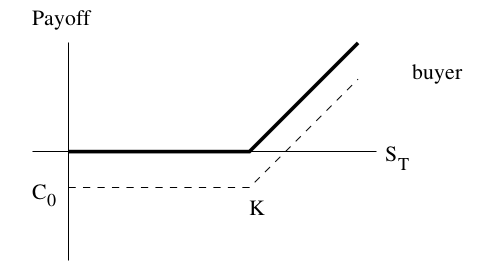
\includegraphics[width=1\linewidth]{Buyer_call} 
		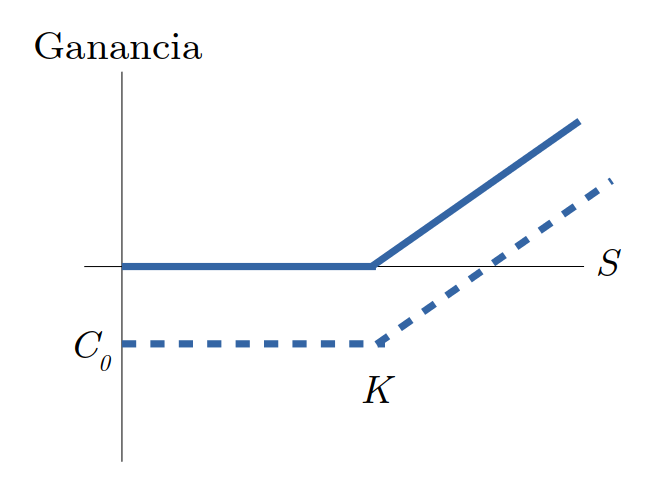
\includegraphics[width=1\linewidth]{Buyer_call_mio} 
		\caption*{Propietario}
		%\label{fig:subim1}
	\end{minipage}
	\begin{minipage}{0.5\textwidth}
		%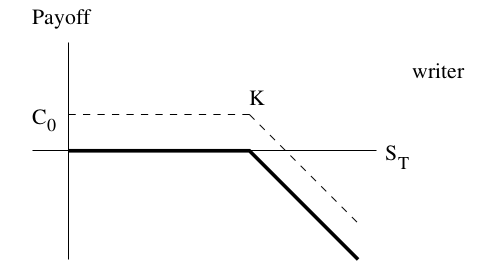
\includegraphics[width=1\linewidth]{Writer_call}
		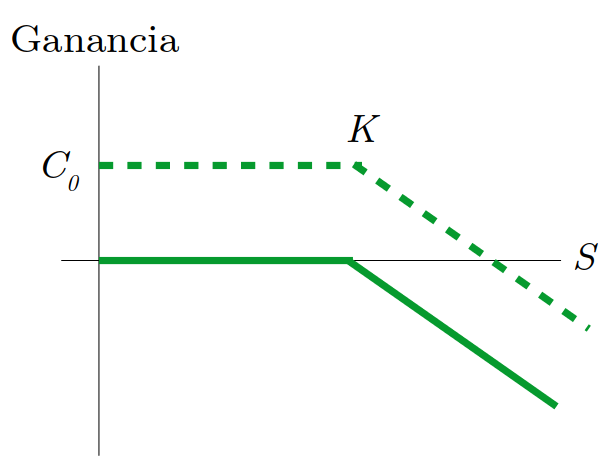
\includegraphics[width=1\linewidth]{Writer_call_mio}
		\caption*{Vendedor}
		
		%\label{fig:subim2}
	\end{minipage}
	
	\caption{Ganancia opción \textit{call}.}
\end{figure}

\begin{figure}[h!]\label{graphPut}
	
	\begin{minipage}{0.5\textwidth}
		\centering
		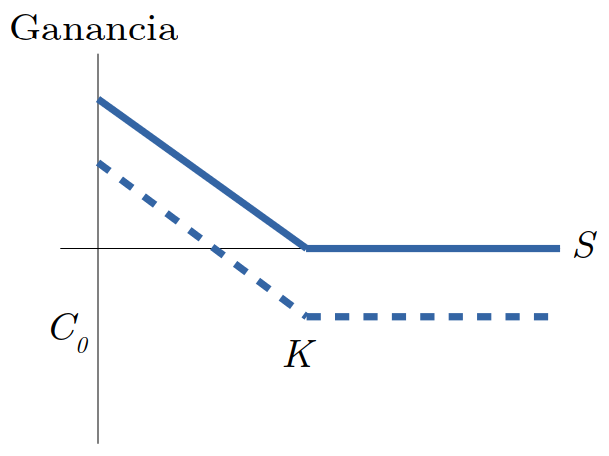
\includegraphics[width=1\linewidth]{Buyer_put_mio} 
		\caption*{Propietario}
		%\label{fig:subim1}
	\end{minipage}
	\begin{minipage}{0.5\textwidth}
		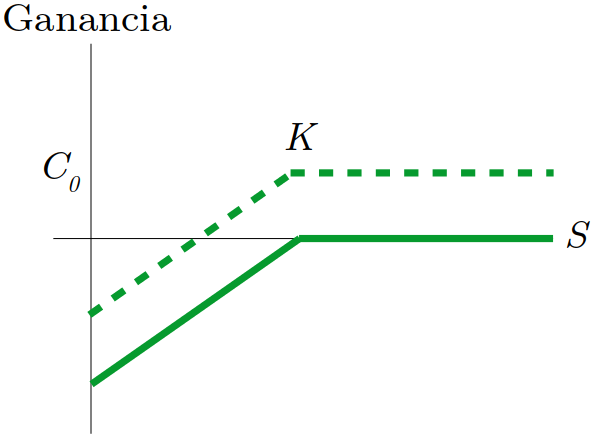
\includegraphics[width=1\linewidth]{Writer_put_mio}
		\caption*{Vendedor}
		%\caption{Tras cuatro iteraciones.}
		
		%\label{fig:subim2}
	\end{minipage}
	
	\caption{Ganancia opción \textit{put}.}
\end{figure} 
Uno de los problemas más importantes es determinar de manera única el precio ``justo'' de una opción en un momento determinado para que ambas partes estén de acuerdo.\\

Una vez explicada de manera simplificada el contexto financiero debemos formalizar matemáticamente modelo del mercado. Fijamos el conjunto de las marcas de tiempo $ \mathbb{T} = \{0,1,\dots,T\}$ con $ T $ el instante en el que finaliza el modelado de nuestra actividad económica. También fijamos el espacio de probabilidad $ (\Omega, \mathcal{F}, P) $. Este espacio contiene todos los posibles estados del mercado. La información de la que disponen los inversores acerca de la estructura en cada momento $ t \in \mathbb{T}$ viene dada por una secuencia finita y creciente de sub-$ \sigma $-álgebras de $ \mathcal{F} $, $ \mathcal{F}_0 \subset \cdots \subset \mathcal{F}_T = \mathcal{F} $ con $ \mathcal{F}_0 $ trivial, es decir, contiene solamente conjuntos con medida 0 o 1. A este secuencia se le denomina filtración y se denota como $ \mathbb{F} = (\mathcal{F}_t)_{t \in \mathbb{T}} $. El sentido financiero de esta filtración es indicar la información conocida hasta el momento acerca de la evolución de los precios. Por ejemplo, si comenzamos a modelar nuestro mercado hoy, $ \mathcal{F}_0 $ nos aporta únicamente el valor actual. Sin embargo, mañana tendremos la información de los precios en ese momento junto con la obtenida hoy, por lo que es claro que $ \mathcal{F}_1 \subset \mathcal{F}_0  $. También es claro que al llegar al instante final tenemos toda la información acerca del modelo. Llamamos $ d  $ a la dimensión de nuestro mercado, es decir, el número de activos que manejamos. La evolución de los precios de los activos viene dada  por el proceso estocástico $ S = \{S^i_t:\hspace{1mm} t \in \mathbb{T},\hspace{1mm} i=0,\dots,d\} $ donde cada $ S^i_t $ es una variable aleatoria. Todos son activos con riesgos menos el marcado por $ 0 $. Asumimos que este proceso se adapta a la filtración $ \mathbb{F} $, es decir, para cada $ t \in \mathbb{T} $ se conocen los precios de cada activo hasta ese instante como se ha explicado anteriormente. En ese caso, decimos que $ S_t^i $ es $ \mathcal{F}_t $-medible para $ i=0,\dots,d $. En general, primero se escoge $ S $ y se toma $ \mathbb{F} $ como la filtración que genera. La tupla $ (\Omega, \mathcal{F}, P, \mathbb{F}, S) $ es la que modela nuestro mercado de valores. \\

El poder adquisitivo de una misma cantidad decrece con el tiempo, consideramos el factor de descuento (o de actualización) en el instante $ t $ dado por $ (0 <?) \beta_t < 1 $ y notamos al valor actual como $ \bar{S}_t = \beta_t S_t $. Sin pérdida de generalidad se puede asumir que $ S^0(0) = 1 $ por lo que podemos expresar todas las unidades en función a dicho valor. En ese caso, el factor $ \beta_t = 1/S^0_t $ es la cantidad de dinero que necesitamos para invertir en bonos en el instante 0 para tener una unidad en el instante $ t $. Podríamos considerar que tomar $ S^0(0) = 1 $  es una simple normalización de los precios. \\

La cartera de inversión o portafolio para el instante $ t \in \mathbb{T} $ viene dada por la variable aleatoria $ d+1 $ dimensional $ \theta_t = (\theta_t^0,\dots,\theta_t^d) $. Cada $ \theta_t^i $ indica el número de activos del tipo $ i $ que tiene un inversor en el instante $ t $. El valor de la cartera viene determinado por $ V_t(\theta) $ donde
\[
V_0(\theta) = \langle \theta_1 , S_0\rangle, \hspace{2.5mm} V_t(\theta) = \langle \theta_t , S_t\rangle = \sum_{i=0}^{d} \theta_t^i S_t^i \text{ para } \hspace{0.5mm} t \in \mathbb{T}, t \geq 1.
\]
Cada inversor seleccionan la cartera de inversión del instante $ t $ una vez se conocen los precios del momento anterior $ t-1 $. La estrategia de inversión $ \theta = \{\theta_t: \hspace{0.5mm}t=1,\dots,T\} $ es el conjunto de todas las carteras de inversión \textit{predecibles}. Decimos que una cartera $ \theta_{t} $ es predecible si depende solamente de los precios de los activos hasta el instante $ t-1 $. Cuando cada cartera de inversión $ \theta_{t+1} $ se puede financiar completamente con las ganancias o pérdidas actuales decimos que la estrategia es \textit{autofinanciada}, es decir, 
\begin{equation*}\label{selfinance}
\langle \theta_{t+1}, S_t \rangle = \langle \theta_{t}, S_t \rangle,
\end{equation*} Notamos $ \Delta X_t = X_t - X_{t-1} $ para cualquier función sobre $ \mathbb{T} $. Si una cartera es autofinanciada, escribimos la ganancia de una cartera de inversión entre los instantes $ (t-1,t] $ como 
\[
\Delta V_t(\theta) = \langle\theta_t, S_t \rangle - \langle\theta_{t-1}, S_{t-1}\rangle = \langle\theta_t, S_t \rangle - \langle\theta_{t}, S_{t-1}\rangle = \langle\theta_{t}, \Delta S_{t}\rangle.
\]
De este modo, la ganancia asociada a la estrategia $ \theta $ hasta el instante $ t $ viene dada por
\[
G_0(\theta) = 0, \hspace{2.5mm} G_t(\theta) = \langle\theta_{1}, \Delta S_{1}\rangle + \cdots + \langle\theta_{t}, \Delta S_{t}\rangle \text{ para } \hspace{0.5mm} t \in \mathbb{T}, t \geq 1.
\]
Vemos entonces que una estrategia es autofinanciada si, y solo si
\begin{equation}\label{selfinifonlyif}
V_t(\theta) = V_0(\theta) + G_t(\theta), \hspace{1mm} \forall t \in \mathbb{T}.
\end{equation}

Destacamos que todas la definiciones anteriores se pueden definir también en base a los valores actualizados $ \bar{S}_t $. \\

También es necesario imponer o aclarar una serie de suposiciones sobre nuestro modelo financiero:
\begin{enumerate}
	\item Ninguna de las transacciones conlleva un coste extra.
	\item Positividad: todos los precios son positivos, es decir,
	\[
	S_t^i > 0 \text{ para } t \in \mathbb{T},\hspace{1mm} i=0,\dots,d.
	\]
	\item Divisibilidad, liquidez y \textit{short selling}: el número de activos que posee un inversor puede ser cualquier valor real. Así,
	\[
	\theta_t^i \in \RR \text{ para } t \in \mathbb{T},\hspace{1mm} i=0,\dots,d.
	\]
	La divisibilidad hace referencia a que $ \theta_t^i $ puede ser una fracción. Claramente, no podemos tener, po ejemplo, media acción. Sin embargo, cuando estamos trabajando con un gran número de acciones podemos considerar que tienen cifras decimales para trabajar con números menores. El hecho de que tome valores en $ \RR $ también significa que podemos comprar o vender el número de acciones deseado, es decir, no imponemos ninguna restricción. Este hecho se conoce como liquidez. Claramente, en mercados reales sí existe dicha restricción en el volumen de las transacciones pero nosotros estamos trabajando con un modelo idealizado. Finalmente, cuando dichos valores son positivos decimos que el inversor tiene una posición larga o \textit{long position}. Si por el contrario estos son negativos, tiene una posición corta o \textit{short position}, por ejemplo, cuando vende algún tipo de bono. Estas acciones se suelen llevar a cabo, por ejemplo, en las denominadas ventas en corto o \textit{short selling} que se usan cuando se prevé que un determinado activo va a bajar de valor. Así, suponemos que tenemos una acción cuyo precio actual es 100 cuyo valor suponemos que va a disminuir. Antes de que baje más, la vendemos, es decir, tomamos una posición \textit{short}. Pasado un periodo de tiempo, la acción bajan a 70 por lo que tomamos una posición \textit{long} y las compramos de nuevo. De este modo, tenemos las misma cantidad de activos que al principio pero hemos obtenido un beneficio de 70. En estas operaciones también corremos el riesgo de perder dinero ya que es posible que el valor de los activos crezca en vez de disminuir. 
	
	\item Solvencia: el valor de todas las carteras las carteras de inversión debe ser siempre positivo,
	\[
	V_t (\theta) \geq 0\text{ para todo } t \in \mathbb{T}.
	\]
	En este caso, decimos que la cartera es \textit{admisible}. A la clase de estrategias autofinanciadas y admisibles la denotaremos como $ \Theta_a $.
	\item El espacio $ \Omega $ es finito, es decir, las variables aleatorias $ S_t^i $ no pueden tomar infinitos valores. Así, tenemos que $ \Omega = \{ \omega_1,\dots,\omega_n\} $.
\end{enumerate}

Ya tenemos el modelo financiero sobre el que vamos a trabajar. Exponemos ahora unos resultados que nos servirán posteriormente para probar el teorema principal del trabajo.

%% Parecido Prop 4.1 del otro libro Mathematics for finance
%% LEMMA 2.2.1
\begin{lemaBox}\label{2.2.1}
	Dada $ V_0 $ una función $ \mathcal{F}_0 $-medible y para $ d \in \NN  $ sean los procesos reales y predecibles $ \theta^1,\dots,\theta^d $ , el único proceso predecible $ \theta^0 $ que convierte a $ \theta = (\theta^0,\theta^1,\dots,\theta^d) $ en una estrategia autofinanciada con valor $ V_0 (\theta)= V_0 $ viene dado por
	\[
	\theta^0_t = V_0 + \sum_{i=1}^{t-1}(\theta^1_i\Delta\bar{S}^1_i+\cdots+\theta^d_i\Delta\bar{S}^d_i) - (\theta^1_t\bar{S}^1_{t-1}+\cdots+\theta^d_t\bar{S}^d_{t-1}).
	\]
\end{lemaBox}
\begin{proof}
	Claramente $ \theta^0 $ es predecible. Para ver que la estrategia es autofinanciada, por \eqref{selfinifonlyif} solo necesitamos ver que $ \theta^0_t $ es la única solución predecible de la ecuación 
	\begin{equation*}
	\begin{split}
	\bar{V}_t(\theta) &= \theta^0_t + \theta^1_t\bar{S}^1_t+\cdots+\theta^d_t\bar{S}^d_t \\
	&= V_0 + \sum_{i=1}^{t}(\theta^1_i\Delta\bar{S}^1_i+\cdots+\theta^d_i\Delta\bar{S}^d_i)
	\end{split}
	\end{equation*}
\end{proof}

Introducimos ahora el concepto de \textit{viabilidad} necesario para el siguiente resultado. Decimos que un mercado es viable si para toda estrategia admisible y autofinanciada no contiene ninguna oportunidad de arbitraje. La ausencia de arbitraje significa que si el valor inicial de una cartera de inversión es $ V_0(\theta) = 0 $ entonces $ V_T(\theta) = 0 $ con probabilidad 1 para toda $ \theta \in\Theta_a $. 

%% LEMMA 3.2.1
\begin{lemaBox}\label{3.2.1}
	Si el modelo de mercado es viable, las ganancias actualizadas a cualquier proceso predecible $ \hat{\theta} \in \RR ^d $ no pueden pertenecer a 
	\[
	C = \{Y \in \RR^n: Y_i \geq 0\text{ para } i=1,\dots,n \text{ y } \exists i \text{ tal que } Y_i > 0\}.
	\]
\end{lemaBox}
\begin{proof}
En primero lugar vemos que $ C $ es el octante positivo de $ \RR^n $ sin el origen que claramente es un cono y es convexo. La ausencia de arbitraje significa que para toda estrategia admisible $ \theta \in \Theta_a $ tal que $ V_0(\theta) = 0 $ entonces
\[
\bar{V}_t(\theta) = \bar{G}_t (\theta) \notin C.
\]
Por el lema \ref{2.2.1}, dados los procesos predecibles $ \hat{\theta} = (\theta^1, \dots,\theta^d) $, existe un único proceso real $ \theta^0 $ tal que $ \theta = (\theta^0, \theta^1,\dots, \theta^d) $ es autofinanciada y $ V_0(\theta) = 0 $. Las ganancias con los valores actualizados viene dada por
\[
\bar{G}_t(\hat{\theta}) = \sum_{j=1}^{t} \langle \theta_j, \Delta \bar{S}_j \rangle =   \sum_{j=1}^{t} \left( \sum_{i=1}^{d} \theta_j^i \Delta \bar{S}_j^i  \right).
\]
Supongamos que $ \bar{G}_t(\hat{\theta}) \in C $, si $ \beta_T $ denota el factor de descuento en el instante $ T $,
\[
V_T(\theta) = \beta_T^{-1} \bar{V}_T(\theta) = \beta_T^{-1}(V_0 (\theta) + \bar{G}_T(\theta)) = \beta_T^{-1}\bar{G}_T(\theta).
\]
Vemos entonces que $ V_T(\theta) $ es no negativa y estrictamente positiva con probabilidad no nula, lo que contradice la viabilidad al existir arbitraje.
\end{proof}

Nuestro objetivo es caracterizar la viabilidad de un mercado en términos de los incrementos de $ \bar{S} $. Para ello son necesarias las martingalas.
\begin{definicion}
Un proceso $ \mathbb{F} $-adaptado $ M = (M_t)_{t\in \mathbb{T}} $ es una $ ( \mathbb{F},P) $-martingala si $ E(|M_t|) < \infty $ para todo $ t \in \mathbb{T} $ y 
\[
E(M_{t+1}|\mathcal{F}_t) = M_t \textit{ para todo } t \in \mathbb{T}\setminus{T}.
\]
Si $ M = (M_t) $ es una martingala y $ \phi = (\phi_t)_{t\in \mathbb{T}} $ es un proceso predecible en $ (\Omega, \mathcal{F}, P, \mathbb{F}, S) $ entonces al proceso $ X = \phi \cdot M $ dado por
\[
X_0=0, \hspace{2mm}X_t = \phi_1\Delta M_1+\cdots+ \phi_t\Delta M_t \hspace{1.5mm} t \geq1
\]
se le denomina martingala transformada de $ M $ por $ \phi $.
\end{definicion}

Notamos que $ M $ es una martingala si, y solo, si
\[
E(\Delta M_{t+1} |\mathcal{F}_t ) = 0 \text{ para todo } t\in \mathbb{T}\setminus\{T\}.
\]
También es importante destacar que, por la linealidad de la esperanza, cualquier combinación lineal de martingalas es una maartingala. \\

Que los precios en el mercado sigan una martingala no debe de ser extraño. Recordemos que para $ t \in \mathbb{T} $, $ \mathcal{F}_t $ indica la cantidad de información acerca de los precios de los activos hasta dicho momento. Por lo tanto, la esperanza condicionada solo nos indica que estamos calculando el valor esperado a partir de lo que conocemos hasta ahora. Además, para que el mercado sea ``justo'', dicho valor en el futuro debería ser, en media, el que tenemos ahora. \\

EXPLICAR MARTINGALAS TRANSFORMADAS + INTEGRABILIDAD. \\

%% THEOREM 2.3.5
\begin{teoremaBox}\label{2.3.5}
	Un proceso real $ M $ es una martingala si, y solo si, 
	\[
	E((\phi \cdot M)_t) = E(\sum_{i=1}^{t}\phi_i\Delta M_i) = 0, \hspace{1mm} \forall t \in \mathbb{T}\setminus\{0\}
	\]
	para todo proceso $ \phi $ predecible y acotado.
\end{teoremaBox}
\begin{proof}
	Si $ M $ es un martingala, también lo es la tranfomada $ X = \phi \cdot M $ y $ X_0 =0 $ ya que
	\[
	E(\Delta X_{t+1}|\mathcal{F}_t) = E(\phi_{t+1}\Delta M_{t+1}|\mathcal{F}_t) =  \phi_{t+1} E(\Delta M_{t+1}|\mathcal{F}_t) = 0.
	\] 
	Por ello, $ E((\phi \cdot M)_t) = 0 $ para todo $ t \geq 1 $ en $ \mathbb{T} $.
	Demostremos ahora la otra implicación. Para $ s > 0 $, sea $ A \in \mathcal{F}_s $ y definimos el proceso predecible $ \phi $ como $ \phi_{s+1} = 1_A $ y $ \phi_t = 0 $ para el resto de $ t\in \mathbb{T} $. Entonces, para $ t > s $ se tiene que
	\[
	0 = E((\phi \cdot M)_t) = E(1_A(M_{s+1}-M_s)).
	\]
	Como es cierto para todo $ A \in \mathcal{F}_s $, se cumple que $ E(\Delta M_{s+1} | \mathcal{F}_s) = 0 $ por lo que $ M $ es una martingala.
\end{proof}

Nos encontramos ahora un contexto general donde no asumimos que el modelo sea finito o que $ \mathbb{F} $ sea generada por $ S $. Supongamos que el proceso de los precios actualizados $ \bar{S} $ es una martingala bajo una probabilidad $ Q $, esto es:
\[
E_Q (\Delta \bar{S}^i_t | \mathcal{F}_{t-1}) = 0, \text{ para } t \in \mathbb{T}\setminus \{0\} \text{ e } i = 0,\dots,d.
\]
Sea $ \theta \in \Theta_a $ una estrategia admisible tal que los procesos de los precios actualizados son integrables respecto a $ Q $, por \eqref{selfinifonlyif} tenemos que:
\begin{equation*}
\begin{split}
\bar{V}_t(\theta) &= V_0(\theta) + \bar{G}_t(\theta) \\
&= \langle \theta_{1}, S_0 \rangle + \sum_{u=1}^{t} \langle \theta_{u}, \Delta \bar{S}_u \rangle \\
&= \sum_{i=1}^{d}(\theta_1^i S_0^i + \sum_{u=1}^{t} \theta_{u}^i \Delta \bar{S}_u^i).
\end{split}
\end{equation*}
Vemos entonces que $ \bar{V}(\theta) $ es una constante más una suma finita de martingalas transformadas, por lo que también es una martingala con valor inicial $ V_0 (\theta) $. Entonces, tenemos que: \[ E(\bar{V}_t (\theta)) = E(V_0 (\theta)) = V_0(\theta) .\] 
Esta situación imposibilita la existencia de arbitraje. Si sabemos de antemano que los procesos de los precios actualizados son integrables respecto a $ Q $, supongamos que $ V_0 (\theta) = 0$ y $ V_T (\theta) \geq 0$ casi seguramente (respecto a $ Q $). Como $ E_Q = (\bar{V}_t ( \theta)) = 0 $ se sigue que $ V_T(\theta) = 0$ casi seguramente (respecto a $ Q $). Esto sigue siendo verdadero casi seguramente para $ P $, demostrando que $ P $ y $ Q $ tienen los mismos conjuntos vacíos. Llegamos entonces a la siguiente definición:
\begin{definicion}
Una probabilidad $ Q $ que sea equivalente a $ P $ $ (Q\sim P) $ es una medida martingala equivalente (EMM) para $ S $ si el proceso de los precios actualizados $ \bar{S} $ es una martingala bajo $ Q $ para la filtración $ \mathbb{F} $. Es decir, para cada $ i =0,\dots, d $ tenemos que $ \bar{S}^i $ es una $ (\mathbb{F},Q) $-martingala.
\end{definicion}

Todo lo presentado anteriormente, nos aporta el siguiente resultado que ya se ha demostrado:
\begin{proposicionBox}\label{martThenViab}
Si existe una medida martingala equivalente para $ S $, entonces el modelo de mercado discreto es viable, es decir, no contiene ninguna oportunidad de arbitraje.	
\end{proposicionBox}

Exponemos ahora el siguiente teorema que es el objetivo final de este trabajo y en el que usaremos las herramientas que hemos ido desarrollando anteriormente.
\begin{teoremaBox}\label{VIABLEiofEMM}
	Un modelo de mercado discreto es viable si, y solo si, existe una medida de martingala equivalente para $ S $.
\end{teoremaBox}
\begin{proof}
	Ya sabemos por la proposición \ref{martThenViab} que la existencia de una medida de martingala equivalente garantiza la viabilidad del modelo por lo que solo tenemos que probar la otra implicación. \\
	
	Suponemos entonces que el modelo es viable. Necesitamos construir una medida $ Q \sim P $ en la que los precios son martingalas relativas a la filtración $ \mathbb{F} $. Recordamos que $ C $ es el cono convexo de todas las variables aleatorias reales $ \phi $ en $ (\Omega, \mathcal{F}) $ tales que $ \phi(\omega) \geq 0 $ casi seguramente y $ \phi(\omega_i) > 0 $ para al menos un $ \omega_i = \Omega = \{\omega_i,\dots, \omega_n \} $. Asumimos $ p_i = P(\{\omega_i\}) > 0 $. Por el lema \ref{3.2.1}, hemos visto que para un mercado viable debemos tener $ \bar{G}_t(\hat{\theta}) \notin C$ para todos los procesos predecibles $ \hat{\theta} \in  \RR^d $. Por otro lado, el conjunto definido por tales ganancias 
	\[
	L = \{\bar{G}_t(\hat{\theta}):\hspace{0.5mm} \hat{\theta}=(\theta^1,\dots,\theta^d),\text{ con } \theta^i \text{ predecible para } i=1,\dots,d \},
	\]
	es un subespacio vectorial del espacio de todas las funciones reales y  $ \mathcal{F} $-medibles en $ \Omega $. Como $ L $ y $ C $ son disjuntos, podemos separar $ L $ y el subconjunto compacto de $ C $ definido como $ K =\{X\in C: \hspace{0.5mm} E_P(X) = 1\} $ mediante el corolario \ref{coroSep}. Sea $ \xx^0 \in \RR^d $ el elemento que proporciona dicho resultado. Tomamos $ \xi_i = (0,\dots,\frac{1}{p_i},\dots,0) $ para $ i \leq n $. Vemos que $ E_P(\xi_i) = \frac{p_i}{p_i} = 1$ por lo que $ \xi_i \in K $ y por ello $ \langle \xx^0, \xi_i \rangle = \frac{x^0_i}{p_i} > 0$. Por ello, $ x^0_i > 0$ para todo $ i=1,\dots,n $.
	
	Definimos ahora el funcional lineal $ g(\xx) = \frac{\langle \xx^0, \xx\rangle}{\alpha} $ donde $ \alpha = \sum_{i=1}^{n} x^0_i$. Sea $ p^* \in \RR^d$ un vector con $ p^*_i = \frac{x_i^0}{\alpha} $ por lo que $ \sum_{i=1}^{n} p^*_i = 1 $. Usamos el vector $ p^* $ para inducir una probabilidad $ P^* $ en $ \Omega = \{\omega_1,\dots,\omega_n\} $ haciendo $ P^*(\{\omega_i\}) = p^*_{i} > 0 $. Veamos que $ P^* $ es la martingala equivalente deseada. En efecto, sea $ E^*(\cdot) $ que denota la esperanza relativa a $ P^* $. Nuevamente, por el corolario \ref{coroSep}, tenemos que $ g(\xx) = \frac{1}{\alpha}\langle \xx^0,\xx\rangle = 0$ para todo $ \xx\in L $. En particular, esta situación se da para  para $ \bar{G}_T (\hat{\theta}) $ con $ \hat{\theta}=(\theta^1,\dots,\theta^d) $ un vector de procesos predecibles por lo que.
	\[ E^*(\bar{G}_T (\hat{\theta})) = 0.\]
	 Hemos una estrategia auto-financiada $ \theta $ con $ V_0(\theta) = 0 $????????. Como $ \bar{V}_t (\theta) = V_0(\theta) + \bar{G}_T (\theta)$, implica que $ E^*(\bar{V}_t (\theta)) = 0 $ para cada $ \theta $. Por el lema \ref{2.2.1} podemos generar tal $ \theta $ para cada proceso predecible de $ n $  dimensiones (¡TENGO MUCHO JALEO CON LAS DIMENSIONES!). En particular, lo podemos hacer para $ (0,\dots, \theta^i,\dots,0) $ donde $ i\leq n $. Por lo tanto
	\[
	E^*(\sum_{t=1}^{T}\theta_t^i\Delta \bar{S}^i_t) = 0
	\]
	se da para cada proceso predecible y acotado $ (\theta^i)_{i=1,\dots,T} $. El teorema \ref{2.3.5} implica que cada $ S^i $ es una martingala bajo $ P^* $. Por ello, $ P^* \sim P $.
\end{proof}

Usemos toda la información obtenida para llegar a una fórmula que nos permitirá establecer el precio de una opción europea. Para ello, utilizaremos un modelo binomial con más de un paso en el que suponemos que $ d = 1 $. De este modo, tenemos un activo sin riesgo con precios $ S^0 $ y uno con riesgo con precios $ S^1$ los cuales denotaremos po $ S $. También, como mencionamos anteriormente, sin pérdida de generalidad asumimos que $ S^0_0  = 1$ por lo que $ S_t^0 =  (1+r)^t $ para $ t \in \mathbb{T} $. El factor de actualización sería en este caso $ \beta_t = (1+r)^{-t} $. Los precios de nuestro activo con riesgo viene determinados por $ S_{t-1}(1+u) $ o $ S_{t-1}(1+d) $ cumpliendo $ -1 < d < u $. El valor inicial $ S_t $ es constante y conocido. Tomamos entonces como espacio de probabilidad $ \Omega = \{1+u,1+d\}^T $ con la filtración $ \mathbb{F} $. Por ello, $ \mathcal{F}_0 = \{\emptyset, \Omega\} $ y $ \mathcal{F}_t = \sigma(S_u^1: \hspace{1mm} u \leq t) $ para $ t >0 $. Para $ \omega = \{\omega_1,\dots,\omega_n\} $ en $ \Omega $ definimos
\[
P(\{\omega\}) = P(\frac{S_t}{S_{t-1}} = \omega_t, \hspace{1mm} t=1,\dots,T).
\]
Notamos a $ \frac{S_t}{S_{t-1}} $ como $ R_t $. Veamos la relación necesaria entre $ a,b \text{ y } r$ para que tengamos una medida martingala equivalente.
\begin{lemaBox}
Para tener una EMM en el modelo binomial se debe cumplir que $ d < r < u $.
\end{lemaBox}
\begin{proof}
Sea $ Q $ una probabilidad en $ (\Omega, \mathcal{F}) $. Para que sea una martingala equivalente se debe dar:
\[
E_Q(\bar{S}_t | \mathcal{F}_{t-1}) = \bar{S}_{t-1}.
\]
\[
\big\Updownarrow
\]
\[
E_Q(R_t | \mathcal{F}_{t-1} ) = E_Q(\frac{\bar{S}_t}{\bar{S}_{t-1}} | \mathcal{F}_{t-1}) = E_Q(\frac{\beta_t}{\beta_{t-1}} | \mathcal{F}_{t-1}) = \frac{\beta_t}{\beta_{t-1}} = 1+r.
\]
Como $ R_t $ solo puede tomar valores $ 1+u $ y $ 1+d $, su valor medio solo puede $ 1+r $ si, y solo si, $ d < r < u $.
\end{proof}

A continuación, vamos a construir dicha medida $ Q $ mediante el siguiente lema:
\begin{lemaBox}\label{cotasUpDown}
El proceso $ \bar{S} $ es una $ (\mathbb{F},Q) $-martingala si, y solo si, las variables aleatorias $ R_t $ son independientes e idénticamente distribuidas con $ Q(R_1 = 1+u) = \frac{r-d}{u-d}$ y $ Q(R_1 = 1+d) = 1- \frac{r-d}{u-d} $. Además, si el modelo es viable, $ Q $ es única.
\end{lemaBox} 
\begin{proof}
Para simplificar la notación, llamamos $ q =  \frac{r-d}{u-d}$.
\begin{itemize}
\item[$ \Longleftarrow $)] Como $ R_t $ son independientes:
\[
E_Q(R_t | \mathcal{F}_{t-1}) = E_Q(R_t) = q(1+u) + (1-q)(1+d) = q(u-d) + 1 +d = 1+r.
\]
Siguiendo un proceso similar a la demostración del lema \ref{cotasUpDown}, vemos que efectivamente es una $ (\mathbb{F},Q) $-martingala.
\item[$ \Longrightarrow $)] En este caso, $ E_Q(R_t | \mathcal{F}_{t-1}) = 1+r $. Como solo puede tomar valores $ 1+u $ y $ 1+d $, se debe cumplir que
\[
(1+d)Q(R_1 = 1+d | \mathcal{F}_{t-1}) + (1+u)Q(R_1 = 1+u | \mathcal{F}_{t-1}) = 1+r
\]
y
\[
Q(R_1 = 1+d | \mathcal{F}_{t-1}) + Q(R_1 = 1+u | \mathcal{F}_{t-1}) = 1.
\]
Llamando $ q =  Q(R_1 = 1+u | \mathcal{F}_{t-1})$ obtenemos
\[
(1+d)(1-q) + (1+u)q = 1+r \Longrightarrow q = \frac{r-d}{u-d}.
\]
Usamos la inducción para probar la independencia de $ R_t $ con $ t >0 $. Para $ \omega = (\omega_1,\dots,\omega_T) \in \Omega $ vemos que
\[
Q(R_1 = \omega_1,\dots,R_t = \omega_t) = \prod_{i=1}^{t}q_i
\]
donde
\[
q_i =  \begin{cases}
q & \text{ si } \omega_i = 1+u\\
S(0)(1+d) & \text{ si } \omega_i = 1+d
\end{cases}.
\]
Por lo tanto, las variables $ R_t $ son independientes e idénticamente distribuidas.
\end{itemize}

Finalmente veamos la unicidad. Es claro que $ q \in (0,1) $ si, y solo si, $ d<r<u $. Por ello, usando el teorema \ref{VIABLEiofEMM} y el lema \ref{cotasUpDown}, obtenemos que el modelo admite una única EMM que además es $ Q $.
\end{proof}

De este modo, la ganancia $ C_T = \max\{S_T-K, 0\} = \left[S_T - K\right]^+$ de una opción \textit{call} en el instante $ t \in \mathbb{T} $ viene dado por
\[
V_t(C_T) = \frac{1}{\beta_t} E_Q(\beta_T C_T | \mathcal{F}_t).
\]
Usando la definición de $ R_t $, vemos que se cumple la siguiente relación:
\[
S_T = S_t \prod_{u = t+1}^{T}R_u.
\]
Podemos calcular su media ya que $ S_t $ es $ \mathcal{F}_t $-medible y $ R_u $ son independientes de $ \mathcal{F}_t $ si $ u > t $. De ese modo,
\begin{equation*}
\begin{split}
V_t (C_T) &= \frac{\beta_T}{\beta_t}E_Q(\left[S_t\prod_{u=t+1}^{T}R_u - K\right]^+ | \mathcal{F}_t) \\
&= (1+r)^{t-T} E_Q(\left[S_t\prod_{u=t+1}^{T}R_u - K\right]^+| \mathcal{F}_t) \\
& = (1+r)^{t-T} \sum_{v=0}^{T-t}\binom{T-t}{v}q^v(1-q)^{T-t-v}\left[S_t(1+u)^v(1+d)^{T-t-v}-K\right]^+.
\end{split}
\end{equation*}
Donde en el último paso se ha usado la fórmula \eqref{valorBino}. Finalmente, en el instante 0, el valor de la opción es:
\begin{equation*}
V_0(C_T) = (1+r)^{-T} \sum_{v=A}^{T-t}\binom{T}{v}q^v(1-q)^{T-v}\left[S_0(1+u)^v(1+d)^{T-v}-K\right],
\end{equation*}
donde $ A $ denota el primer entero $ k $ que cumple $ S_0(1+u)^k(1+d)^{T-k} > K $. Esto se debe a que \[\left[S_0(1+u)^j(1+d)^{T-j}-K\right]^+ = 0, \hspace{1mm}\text{ para } j<k.\]